\documentclass{beamer}
\mode<presentation>

\usepackage{pgfpages}
\usepackage{bbm}
\usepackage{amsmath}
\usepackage{amssymb} 
\usepackage{amsthm}
\usepackage{epsfig}
\usepackage{graphicx}
\usepackage{natbib}

\graphicspath{{./figures/}}

\makeatletter 
\def\newblock{\beamer@newblock} 
\makeatother  

% set color and font of frametitles
\setbeamercolor{frametitle}{fg=blue}
%\setbeamerfont{frametitle}{series=\bfseries}

\newcommand{\red}[1]{{\color{red} #1}}
\newcommand{\blue}[1]{{\color{blue} #1}}
\newcommand{\avg}[1]{\left\langle #1 \right\rangle}

\newcommand{\code}[1]{{\fontfamily{pcr}\selectfont \textbf{#1}}}

%%%%%%%%%%%%%%%%%%%%%%%%%%%%%%%%%%%%%%%%%%%%%%%%%%%%%%%%%%%%%%%%%
%% SETTINGS

% set item type and color
\setbeamercolor{item}{fg=black}  % set color
\setbeamertemplate{itemize items}[circle] % if you want a circle
\setbeamertemplate{itemize subitem}[ball] % if you wnat a ball
\setbeamertemplate{itemize subsubitem}[triangle] % if you want a triangle

% set spacing for itemize
\setbeamertemplate{itemize/enumerate subbody begin}{\vspace{0.1cm}}
\setbeamertemplate{itemize/enumerate subbody end}{\vspace{0.1cm}}

%% END SETTINGS
%%%%%%%%%%%%%%%%%%%%%%%%%%%%%%%%%%%%%%%%%%%%%%%%%%%%%%%%%%%%%%%%%%%

% remove navigation symbols
\beamertemplatenavigationsymbolsempty 

\title{Version control management and research collaboration using git and github}
\subtitle{An introduction}
\author{APSIS group}
\institute{MCC Berlin}
\date{July 11th, 2019}

\AtBeginSection[]
  {
     \begin{frame}<beamer>
     \frametitle{}
     \tableofcontents[currentsection]
     \end{frame}
  }

\begin{document}

\maketitle


\section{What is git and GitHub?}

% ==============================================================
\begin{frame}
\frametitle{What is version control management?}

Software to keep track of the history and different versions of files within project folders

\end{frame}
%--------------------------------------------------------------


% ==============================================================
\begin{frame}
\frametitle{What is git?}

\begin{itemize}
\item git is a program for version control

\item designed for distributed software development

\item created by Linus Torvalds for his work on the Linux kernel
\end{itemize}

Explain idea of a git repository

\end{frame}
%--------------------------------------------------------------

\begin{frame}
\frametitle{What is GitHub?}

Explain the idea of a remote repository

Explain github (and providers of remote repositories like gitlab, bitbucket, SourceForge, Launchpad ...)

\end{frame}


\section{Why should I use it?}

\begin{frame}
\frametitle{Why use version control in research?}

\begin{itemize}
\item getting some order in the mess
\begin{itemize}
\item data
\item software code/scripts
\item manuscripts for papers 
\end{itemize}

\item sharing your code or 

\item collaboration and attribution of work
\end{itemize}

\end{frame}
%--------------------------------------------------------------

\section{How can I use it?}

% ==============================================================
\begin{frame}
\frametitle{Git Workflow (simplest)}

\begin{columns}
	\begin{column}{0.618\linewidth}
		\begin{figure}
			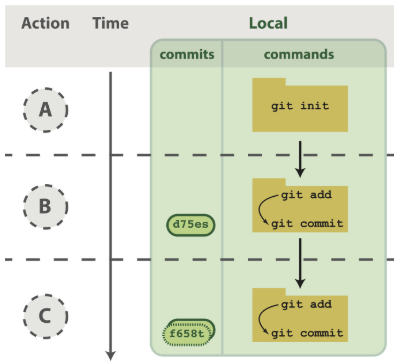
\includegraphics[width=\linewidth]{images/local-workflow}
			\caption{ \cite{Blischak2016}}
		\end{figure}
	\end{column}
	\begin{column}{0.382\linewidth}
		\begin{itemize}
			\item<1-> Keep track of changes in a folder on your computer
			\item<2-> Changes are stored as lines added and removed
			\item<3-> No need to save multiple versions of the same file; you have recorded all changes and can view or revert these at any time
		\end{itemize}
	\end{column}
\end{columns}


\end{frame}
%--------------------------------------------------------------

% ==============================================================
\begin{frame}
\frametitle{Git + Github Workflow (simplest)}

\begin{columns}
	\begin{column}{0.55\linewidth}
		\begin{figure}
			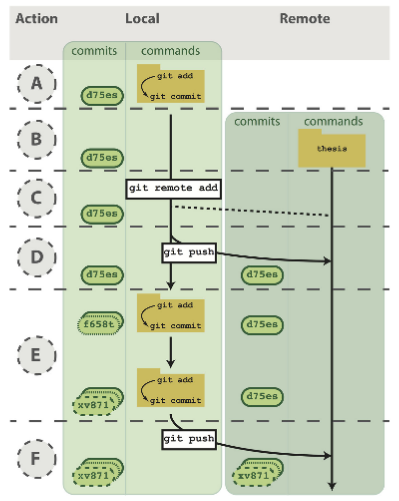
\includegraphics[width=\linewidth]{images/remote-workflow}
		\end{figure}
	\end{column}
	\begin{column}{0.45\linewidth}
		\begin{itemize}
			\item<1-> Attach your repository to a remote version
			\item<2-> If working with collaborators, they also can make a copy (\code{clone}) on their machine
			\item<3-> By both using \code{pull}, you can keep up to date with each others' changes
			\item<4-> For more complicated workflows, especially where maintaining a working version is critical, check out branching \url{https://guides.github.com/introduction/flow/}
		\end{itemize}
	\end{column}
\end{columns}


\end{frame}
%--------------------------------------------------------------



% ==============================================================
\begin{frame}
\frametitle{Tools}

\begin{columns}[t]
	\begin{column}{0.5\linewidth}
		\textbf{Command Line}
		\begin{itemize}
			\item Easy to document/explain
			
			\begin{figure}
				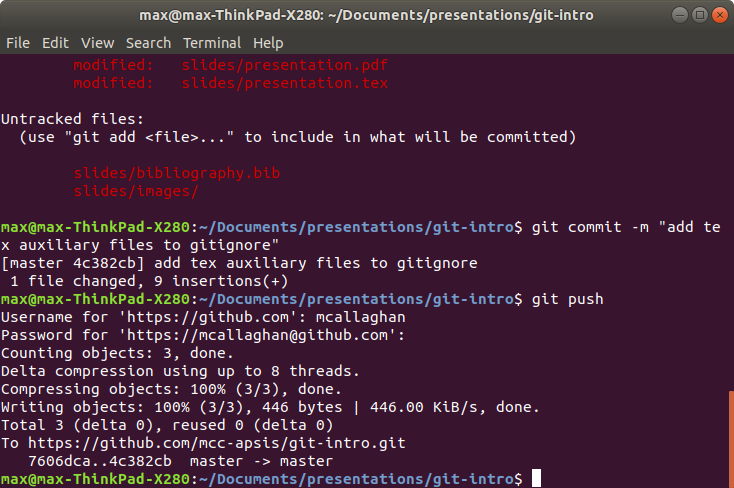
\includegraphics[width=\linewidth]{images/git-terminal}
			\end{figure}
			
			Steeper learning curve, but more flexible and harder to do things unintentionally
		\end{itemize}
	\end{column}

	\begin{column}{0.5\linewidth}
		\textbf{GUIs}
		\begin{itemize}
			\item Easy to use
			
			\begin{figure}
				\includegraphics[width=\linewidth]{example-image}
			\end{figure}
			
			Often there are integrations in development environments, e.g. RStudio, Atom
		\end{itemize}
	\end{column}
\end{columns}



\end{frame}
%--------------------------------------------------------------


% ==============================================================
\begin{frame}
\frametitle{Starting a repository}

To start working with a repository, either turn an existing folder into a git repository

\medskip

\code{git init}

\medskip

or copy an existing repository into a folder

\medskip

\code{git clone}

\end{frame}
%--------------------------------------------------------------

% ==============================================================
\begin{frame}
	\frametitle{Editing a respository}
	
	\begin{itemize}
		\item<1-> Edit files (write some new code or a nice new paragraph)
		
\par\noindent\hrulefill\par
		
		\item<2-> Stage changes (tell git about the changes you want record)
		
		\begin{itemize}
			\item \code{git add -A}
			\item Or add only certain files using patterns or exact file names
		\end{itemize}
		
		\par\noindent\hrulefill\par
		
		\item<3-> Commit changes (make a timestamped version of the repository, recording all the changes you have told git about)
		\begin{itemize}
			\item \code{git commit -m "made a cool new graph"}
			\item It's best if each commit describes a discrete change, and has an interpretable name.
		\end{itemize}
		
		\par\noindent\hrulefill\par
	\end{itemize}
	
	
\end{frame}
%--------------------------------------------------------------

% ==============================================================
\begin{frame}
\frametitle{Managing the repository}

\textbf{Where are we?}

\medskip

\code{git status} tells us which files have changed and are staged or unstaged:

\only{\begin{figure}
	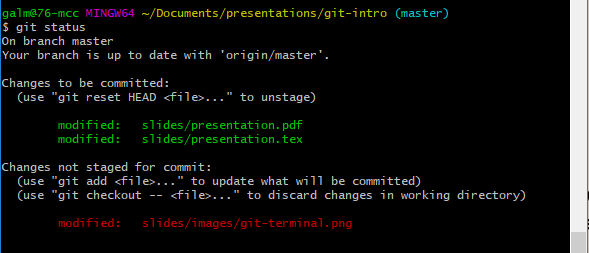
\includegraphics[width=0.8\linewidth]{images/git-status}
\end{figure}}<1>


\par\noindent\hrulefill\par

\textbf{What's changed?}

\code{git diff} lets us know the difference between the files we could stage, and the staged version of them

\only{\begin{figure}
	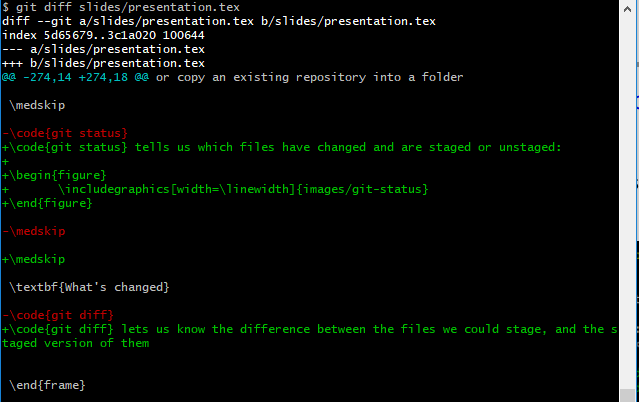
\includegraphics[width=0.8\linewidth]{images/git-diff}
\end{figure}}<2>

\only{\code{git diff} can also tell us about the difference between variously specified versions of files}<3>


\end{frame}
%--------------------------------------------------------------

% ==============================================================
\begin{frame}
	\frametitle{Navigating different versions}
	
	\code{git log} shows us a list of all the commits that have been made.
	
	\only{\begin{figure}
			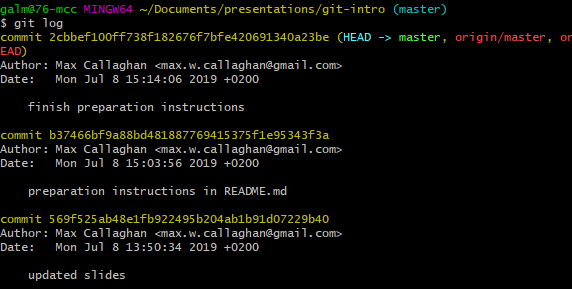
\includegraphics[width=0.8\linewidth]{images/git-log}
	\end{figure}}<1->

\par\noindent\hrulefill\par	

	\code{git checkout}
	
	
\end{frame}
%--------------------------------------------------------------

% ==============================================================
%\begin{frame}
%\frametitle{Branches and merges}
%
%explain what branches are
%
%\code{git branch}
%
%\code{git merge \emph{branchname}}
%
%\code{git checkout}
%
%\end{frame}
%--------------------------------------------------------------

% ==============================================================
\begin{frame}
\frametitle{Interacting with remote repositories}

\code{git pull}

\code{git push}

Warning: careful with copyrighted materials in public repositories

forking and pull request for working on repository for which you are no collaborator

\end{frame}
%--------------------------------------------------------------

% ==============================================================
\begin{frame}
\frametitle{Further useful commands and tools}

.gitignore file

create doi for citations:
https://guides.github.com/activities/citable-code/

\end{frame}
%--------------------------------------------------------------

% ==============================================================
\begin{frame}
\frametitle{}

{\huge
Questions?
}

\end{frame}
%--------------------------------------------------------------

% ==============================================================
\begin{frame}
\frametitle{Practice / task}

\begin{itemize}
\item clone remote repository with

\code{git clone https://github.com/mcc-apsis/git-intro.git}

\item add some question or feedback to the presentation in the file

\item add and commit changes

\item pull changes already made by other

\item push your own changes
\end{itemize}




\end{frame}
%--------------------------------------------------------------


% ==============================================================
\begin{frame}
\frametitle{References}

\bibstyle{unsrt}
\bibliography{bibliography}

\end{frame}
%--------------------------------------------------------------


\end{document}


